\documentclass[a4paper]{article}

\usepackage{graphicx}
\usepackage{caption}
\usepackage{listings}
\usepackage{color}

\definecolor{mygreen}{rgb}{0,0.6,0}
\definecolor{mygray}{rgb}{0.5,0.5,0.5}
\definecolor{mymauve}{rgb}{0.58,0,0.82}

\lstset{ %
  backgroundcolor=\color{white},
  basicstyle=\footnotesize,
  breakatwhitespace=false,
  captionpos=b,
  commentstyle=\color{mygreen},
  frame=single,
  keepspaces=true,
  keywordstyle=\color{blue},
  language=C,
  rulecolor=\color{black},
  stringstyle=\color{mymauve},
  tabsize=2,
  title=\lstname
}

\begin{document}

\title{
Development of Real-Time Systems\\
Assignment 5
}
\author{Elyasin Shaladi}
\maketitle

\tableofcontents
\newpage
\listoftables
\lstlistoflistings
\listoffigures

\newpage

\section{Simulation assignment}
The assignment is to modify a real-time simulator to verify feasibility of a set of tasks.

\subsection{Simulation assignment --- Modification of a real-time simulator}

The partitioned RM scheduler in SimSo is modified to schedule according to a First-Fit algorithm described in the assignment description. Instead of scheduling the task to the CPU with the lowest utilization we chose the first one, which has a lower utilization than $U_{rm}(x+1)$ where x is the already scheduled tasks on the respective CPU.

\begin{table}[!htbp]
\begin{center}
\begin{tabular}{|l||l|l|l|l|}
\hline
Task   & $p_i$ & $e_i$ & $D_i$\\
\hline
\hline
Task 1 & 2 & 1 & 2\\
\hline
Task 2 & 2.5 & 0.1 & 2.5\\
\hline
Task 3 & 3 & 1 & 3\\
\hline
Task 4 & 4 & 1 & 4\\
\hline
Task 5 & 4.5 & 0.1 & 4.5\\
\hline
Task 6 & 5 & 1 & 5\\
\hline
Task 7 & 7 & 1 & 6\\
\hline
Task 8 & 7 & 1 & 7\\
\hline
Task 9 & 8 & 1 & 8\\
\hline
Task 10 & 8.5 & 0.1 & 8.5\\
\hline
Task 11 & 9 & 1 & 9\\
\hline
\end{tabular}
\caption{Tasks T1 to T11}
\end{center}
\end{table}

\subsubsection{Modifying the partitioned RM scheduler}

First I copied and modified the P\_RM.py file and named it P\_RM\_assignment\_5.py.\\
In order for SimSo to recognize the custom scheduler the class name of the partitioned scheduler must correspond to the file name. Therefore we need to modify the line

\begin{lstlisting}[language=Python]
...
class P_RM(PartitionedScheduler):
...
\end{lstlisting}

to

\begin{lstlisting}[language=Python]
...
class P_RM_assignment_5(PartitionedScheduler):
...
\end{lstlisting}

We need to modify the \textit{packer} function and implement the First Fit algorithm. In this First Fit algorithm we assign a task to the first CPU with utilization lower than $U_{rm}(n+1)$ where $n$ is the number of task already assigned to the respective CPU.\\

\begin{lstlisting}[label=First Fit algorithm,caption=Affect a task to the first processor with utilization lower than $U_{rm}$,language=Python]
    def packer(self):
        # First Fit RM
        cpus = [[cpu, 0, 0] for cpu in self.processors]
        for task in self.task_list:
            j = -1

            # Find first the processor with utilization lower
            # than U_rm(n + 1) where n is the number of tasks
            # affected to cpu
            for i, c in enumerate(cpus):
                u = c[1] + float(task.wcet) / task.period
                u_rm = (c[2]+1) * (2**(1/float((c[2]+1))) - 1)
                if u <= u_rm:
                    j = i
                    break

            if j == -1:
                return False

            # Affect it to the task.
            self.affect_task_to_processor(task, cpus[j][0])

            # Update utilization.
            cpus[j][1] += float(task.wcet) / task.period

            # Update number of tasks on cpu
            cpus[j][2] += 1
        return True
\end{lstlisting}

\newpage

Below you can see the result of the scheduling simulation in form of a screen-shot of a Gantt diagram. With this report you'd have also received the SimSo files so that you can perform the simulation yourself.\\
Simply open the file \textit{custom\_scheduler.xml} with SimSo and set the \textit{Scheduler Path} to where the file P\_RM\_assignment\_5.py is located on your machine. \\

\begin{figure}[!ht]
\begin{center}
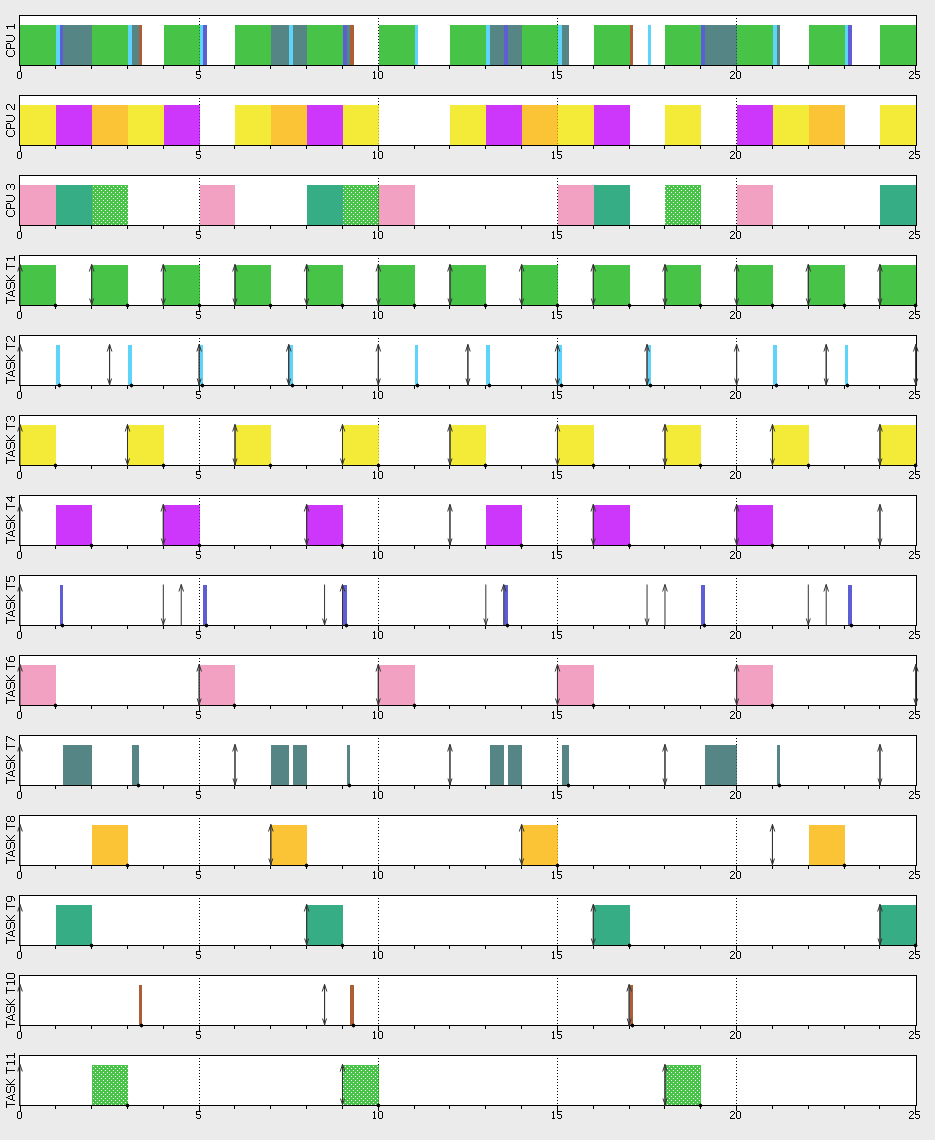
\includegraphics[width=\textwidth]{Gantt_P_RM_First_Fit.png}
\caption{Screen-shot of the Gantt diagram of the simulation}
\end{center}
\end{figure}


\newpage


\section{Programming assignment}

In this programming assignment, we will use message queues in FreeRTOS. \\
We will use the matrix task with the functionality given in the Assignment 5, which is a computationally intensive task, in order to implement the message queue demo. \\
\\
The queue is created in the \textit{main} function with a queue length of 3 and an item size of a pointer, which is a pointer to a \textit{struct}. \\
In the main function the tasks matrix task and reader task are also created. I chose to give both the tasks the same priority.\\

\begin{lstlisting}[label=Creation of tasks and queue,caption=Creation of tasks and queue]
...
// Handles for tasks and queues
xTaskHandle matrix_handle = 0;
xTaskHandle reader_handle = 0;
QueueHandle_t matrix_queue = 0;
...
...
int main(void) {
	/* This demo uses heap_5.c, so start by defining some heap
     regions.  This is only done to provide an example as this
     demo could easily create one large heap region instead of
     multiple smaller heap regions
    */
	prvInitialiseHeap();

	/*FreeRTOS scheduling 1*/
	/*Create the matrix task */
	xTaskCreate((pdTASK_CODE) matrix_task, (signed char * ) "Matrix",
    		1000, NULL, 3, &matrix_handle);
	/*Create the reader task */
	xTaskCreate((pdTASK_CODE) reader_task, (signed char * ) "Reader",
    		1000, NULL, 3, &reader_handle);
	/*Create the matrix queue */
	matrix_queue = xQueueCreate(3, sizeof(struct Message *));

	if (matrix_queue == NULL)
		printf("Failed to create matrix queue.\n");

//This starts the real-time scheduler
	vTaskStartScheduler();
	for (;;)
		;
	return 0;
}
\end{lstlisting}

The structure of the message is simple as it holds only a pointer to a pointer to a double data type:\\

\begin{lstlisting}[label=Message structure,caption=Definition of the Message \textit{struct}]
struct Message {
	double **c;
} xMessage;
\end{lstlisting}

The matrix task is modified so that it sends a message to the message queue before it is put to sleep. The message will contain a the value of the variable \textit{c}, which is a pointer to a pointer to a double data type. \\
Messaging in FreeRTOS is done by copying the values to the message queue as described in the FreeRTOS documentation. So we don't need to deal with data races in this case (the matrix task allocates new memory at each job run).\\
However, concurrency can be a problem in certain cases here. But since it was not required to solve concurrency in this assignment I just skip that step. (A solution would probably be to use semaphores.)\\

\begin{lstlisting}[label=Sending a message,caption=Sending a message to the message queue]
...
		struct Message *pxMessage;
		xMessage.c = c;
		pxMessage = &xMessage;
		if (xQueueSend(matrix_queue, &pxMessage, (TickType_t ) 0)
        		!= pdPASS) {
			printf("Failed to post the message.\n");
			fflush(stdout);
		}
		vTaskDelay(100);
...
\end{lstlisting}

Finally the reader task is defined. The reader task does not block if a message is not immediately available (for this simple example this should be sufficient I think). It keeps polling the queue and when it receives a message then it prints out the data. \\
The rows of the received matrix data is printed out line by line. On small screens it might be a little bit difficult to read. Feel free to modify the output according to your needs.\\

\begin{lstlisting}[label=Reader Task - Receiving a message,caption=Receiving a message from the message queue]
// Reader task to receive from the queue
void reader_task(void *pvParameters) {

	while (1) {
		if (matrix_queue != 0) {
			// Receive a message on the created queue.
			// Don't block if a message is not immediately
			// available.
			struct Message *pxRxedMessage;
			if (xQueueReceive(matrix_queue, &pxRxedMessage,
            		(TickType_t ) 0)) {
				int i, j;
				for (i = 0; i < SIZE; i++) {
					for (j = 0; j < SIZE; j++) {
						printf("[%d][%d] = %.2f ", i, j,
								pxRxedMessage->c[i][j]);
						fflush(stdout);
					}
					printf("\n");
					fflush(stdout);
				}
				printf("\n");
				fflush(stdout);
			}
		}
	}
}
\end{lstlisting}

\newpage

\subsection{Provide a screen-shot of the running system}

I use Eclipse for development. The screen-shot shows the project in execution.\\

\begin{figure}[!ht]
\begin{center}
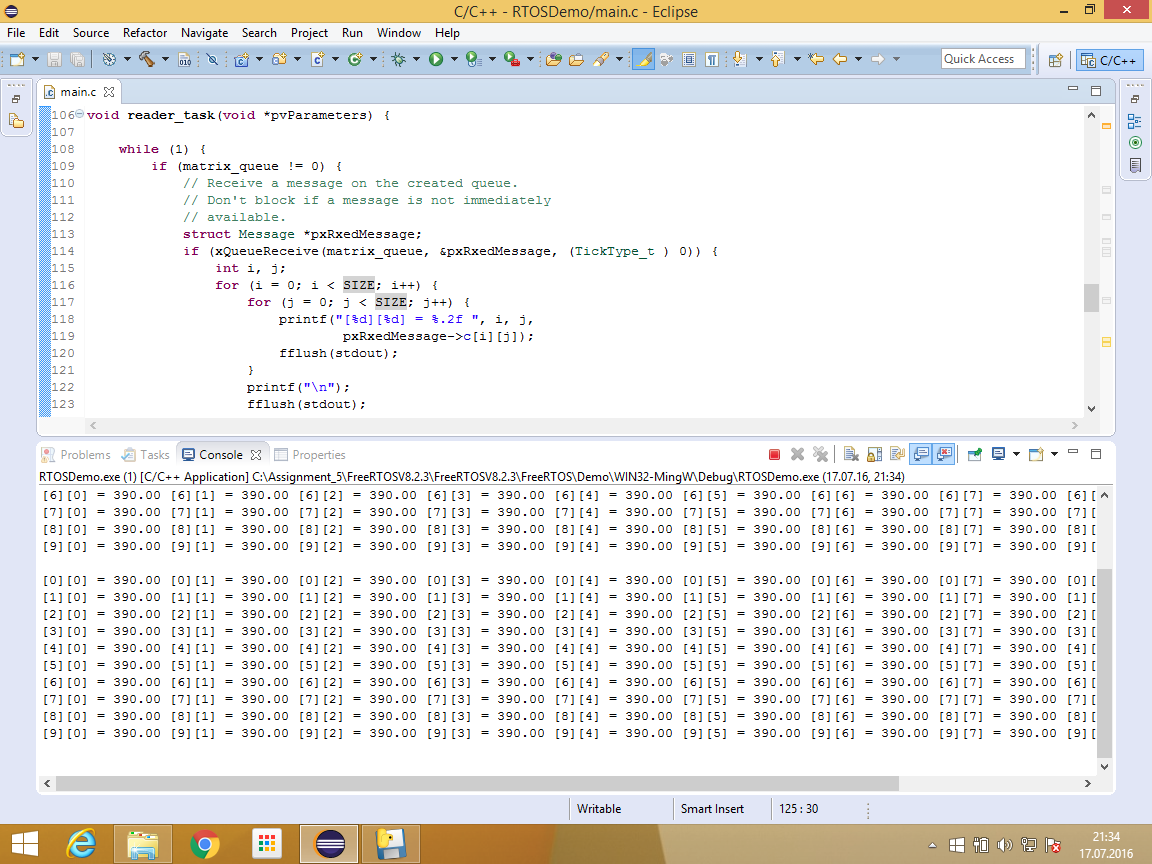
\includegraphics[width=\textwidth]{Assignment_5.png}
\caption{Screen-shot FreeRTOS scheduler execution}
\end{center}
\end{figure}

\end{document}
